\section{常数项级数的概念和性质}
人们认识事物在数量方面的特性,往往有一个由近似到精确的过程.
在这种认识过程中,会遇到由有限个数量相加到无穷多个数量相加的问题.

例如计算半径为\(R\)的圆面积\(A\),具体做法如下:
如\cref{figure:无穷级数.用内接正多边形覆盖圆},
作圆的内接正六边形,算出这六边形的面积\(a_1\),它是圆面积\(A\)的一个粗糙的近似值.
为了比较准确地计算出\(A\)的值,
我们以这个正六边形的每一边为底分别作一个顶点在圆周上的等腰三角形,
算出这六个等腰三角形的面积之和\(a_2\).
那么\(a_1+a_2\)(即内接正十二边形的面积)就是\(A\)的一个较好的近似值.
同样地,在这正十二边形的每一边上分别作一个顶点在圆周上的等腰三角形,
算出这十二个等腰三角形的面积之和\(a_3\).
那么\(a_1+a_2+a_3\)(即内接正二十四边形的面积)是\(A\)的一个更好的近似值.
如此继续下去,内接\(3\cdot2^n\)边形的面积就逐步逼近圆面积:\[
	A \approx a_1 + a_2 + \dotsb + a_n.
\]

\begin{figure}[h]
	\centering
	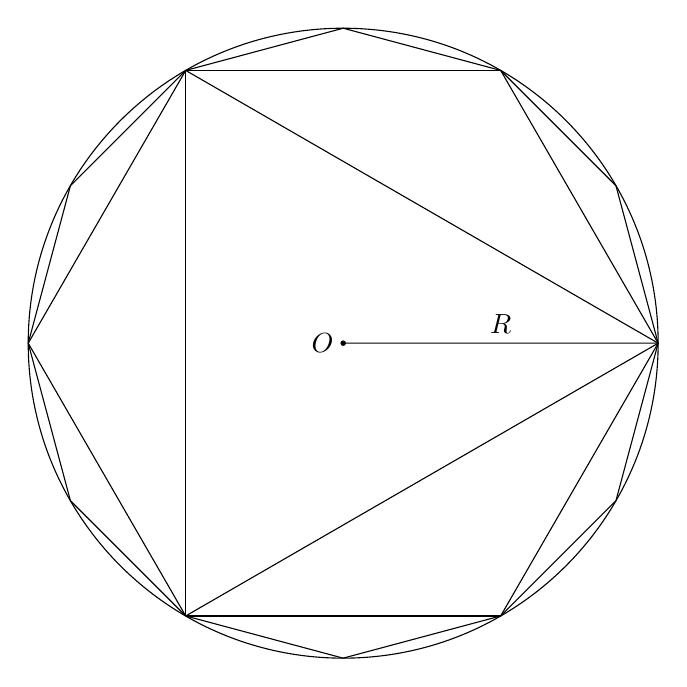
\begin{tikzpicture}
		\pgfmathsetmacro{\radius}{4}
		\def\PlotPolygon#1{
			\foreach \i in {1,...,#1}{
				\draw({\radius*cos(\i*360/#1)},{\radius*sin(\i*360/#1)})
				--({\radius*cos((\i-1)*360/#1)},{\radius*sin((\i-1)*360/#1)});
			}
		}
		\begin{scope}
			\PlotPolygon{3}
			\PlotPolygon{6}
			\PlotPolygon{12}
		\end{scope}
		\draw(0,0)circle(\radius)node[left]{\(O\)}
			--(\radius,0)node[midway,above]{\(R\)};
		\fill(0,0)circle(1pt);

	\end{tikzpicture}
	\caption{用内接正多边形覆盖圆}
	\label{figure:无穷级数.用内接正多边形覆盖圆}
\end{figure}

如果内接正多边形的边数无限增多,即\(n\)无限增大,
则和\(a_1+a_2+\dotsb+a_n\)的极限就是所要求的圆面积\(A\).
这时和式中的项数无限增多,于是出现了无穷多个数量依次相加的数学式子.

\subsection{常数项级数的概念}
\begin{definition}\label{definition:无穷级数.常数项级数的定义}
一般地,给定一个有无穷多项的数列\[
	u_1,u_2,\dotsc,u_n,\dotsc,
\]
则由该数列构成的表达式\[
	u_1+u_2+\dotsb+u_n+\dotsb
\]
叫做\DefineConcept{常数项无穷级数}(infinite series with constant terms),
简称\DefineConcept{常数项级数},
记作\(\sum\limits_{n=1}^\infty u_n\),
即\[
	\sum\limits_{n=1}^\infty u_n
	\defeq
	u_1+u_2+\dotsb+u_n+\dotsb,
\]
其中第\(n\)项\(u_n\)叫做级数的\DefineConcept{一般项}.

作常数项级数的前\(n\)项的和\[
	s_n = u_1+u_2+\dotsb+u_n = \sum\limits_{i=1}^n{u_i}.
\]
我们把\(s_n\)称为级数\(\sum\limits_{n=1}^\infty u_n\)的\DefineConcept{部分和}(partial sum).

如果级数\(\sum\limits_{n=1}^\infty u_n\)的部分和数列\(\{s_n\}\)有极限\(s\),即\[
	\lim\limits_{n\to\infty} s_n = s,
\]
则称“无穷级数\(\sum\limits_{n=1}^\infty u_n\) \DefineConcept{收敛}(converge)”,
这时极限\(s\)叫做这级数的\DefineConcept{和}(sum),并写成\[
	s = u_1+u_2+\dotsb+u_n+\dotsb;
\]
反之,如果\(\{s_n\}\)没有极限,
则称“无穷级数\(\sum\limits_{n=1}^\infty u_n\) \DefineConcept{发散}(diverge)”.

显然,当级数收敛时,其部分和\(s_n\)是级数的和\(s\)的近似值,它们之间的差值\[
	r_n = s - s_n = u_{n+1}+u_{n+2}+\dotsb
\]
叫做“级数\(\sum\limits_{n=1}^\infty u_n\)的\DefineConcept{余项}”.
称这个余项的绝对值\(\abs{r_n}\)为%
“用近似值\(s_n\)代替和\(s\)所产生的\DefineConcept{误差}”.
\end{definition}
从上述定义可知,级数与数列极限有着紧密的联系.给定级数\(\sum\limits_{n=1}^\infty u_n\),
就有部分和数列\(\{s_n = \sum\limits_{i=1}^n u_n\}\);
反之,给定数列\(\{s_n\}\),就有以\(\{s_n\}\)为部分和数列的级数\[
	s_1 + (s_2-s_1) + \dotsb + (s_n-s_{n-1}) + \dotsb
	= s_1 + \sum\limits_{i=2}^\infty (s_i-s_{i-1})
	= \sum\limits_{n=1}^\infty u_n,
\]
其中\(u_1=s_1\),\(u_n=s_n-s_{n-1}\ (n \geq 2)\).
按定义,级数\(\sum\limits_{n=1}^\infty u_n\)与数列\(\{s_n\}\)同时收敛或同时发散,
且在收敛时,有\[
	\sum\limits_{n=1}^\infty u_n = \lim\limits_{n\to\infty} s_n,
\]
即\(\sum\limits_{n=1}^\infty u_n = \lim\limits_{n\to\infty} \sum\limits_{i=1}^n u_n\).

\begin{example}\label{example:无穷级数.等比级数的收敛性}
无穷级数\[
	\sum\limits{n=1} a q^n
	= a+aq+aq^2+\dotsb+aq^n+\dotsb
\]
叫做\DefineConcept{等比级数}或\DefineConcept{几何级数},
其中\(a \neq 0\),\(q\)叫做\DefineConcept{级数的公比}.
试讨论上述等比级数的收敛性.
\begin{solution}
当\(q = 1\)时,则部分和\(s_n=na\),那么\(\lim\limits_{n\to\infty} s_n = \lim\limits_{n\to\infty} na = \infty\),即级数发散.

当\(q \neq 1\),则\[
s_n = \frac{a(1-q^n)}{1-q} = \frac{a}{1-q} - \frac{aq^n}{1-q}.
\]
当\(\abs{q} < 1\)时由于\(\lim\limits_{n\to\infty} q^n=0\),从而\(\lim\limits_{n\to\infty} s_n=\frac{a}{1-q}\),
因此级数收敛,其和为\(\frac{a}{1-q}\).
当\(\abs{q} > 1\)时由于\(\lim\limits_{n\to\infty} q^n=\infty\),从而\(\lim\limits_{n\to\infty} s_n=\infty\),即级数发散.
当\(q = -1\)时,级数变为\(a-a+a-a+\dotsb\),
显然\(s_n\)随着\(n\)为奇数或为偶数而等于\(a\)或等于零,从而\(s_n\)的极限不存在,这是级数也发散.

综上所述,{\color{red}当\(\abs{q} < 1\)时,几何级数收敛;当\(\abs{q} \geq 1\)时,几何级数发散.}
\end{solution}
\end{example}

\begin{example}\label{example:无穷级数.等差级数的收敛性}
试证级数\[
1+2+3+\dotsb+n+\dotsb
\]是发散的.
\begin{proof}
级数的部分和为\[
s_n = 1+2+3+\dotsb+n = \frac{n(n+1)}{2}.
\]显然,\(\lim\limits_{n\to\infty} s_n=\infty\),级数是发散的.
\end{proof}
\end{example}
从上例也可看出:
\begin{proposition}
除非初项\(a_0\)与公差\(d\)都等于\(0\),
否则等差级数\(\sum\limits_{n=0}^\infty(a_0+nd)\)总是发散的.
\end{proposition}

\begin{example}
判定无穷级数\[
\frac{1}{1\cdot2}+\frac{1}{2\cdot3}+\dotsb+\frac{1}{n(n+1)}+\dotsb
\]的收敛性.
\begin{solution}
记\[
	u_n = \frac{1}{n(n+1)} = \frac{1}{n}-\frac{1}{n+1},
\]
因此\begin{align*}
	s_n &= \frac{1}{1\cdot2}+\frac{1}{2\cdot3}+\dotsb+\frac{1}{n(n+1)} \\
	&= \left(1-\frac{1}{2}\right)+\left(\frac{1}{2}-\frac{1}{3}\right)
	+\dotsb+\left(\frac{1}{n}-\frac{1}{n+1}\right) \\
	&= 1-\frac{1}{n+1}.
\end{align*}
从而\[
	\lim\limits_{n\to\infty} s_n = \lim\limits_{n\to\infty} \left(1-\frac{1}{n+1}\right) = 1,
\]
即该级数收敛,它的和为\(1\).
\end{solution}
\end{example}

\subsection{收敛级数的基本性质}
\begin{property}\label{theorem:无穷级数.收敛级数性质1}
如果级数\(\sum\limits_{n=1}^\infty u_n\)收敛于和\(s\),
则级数\(\sum\limits_{n=1}^\infty k u_n\)收敛于和\(ks\).
\begin{proof}
设级数\(\sum\limits_{n=1}^\infty u_n\)
与级数\(\sum\limits_{n=1}^\infty k u_n\)的
部分和分别为\(s_n\)与\(\sigma_n\),
则\[
	\sigma_n
	= k u_1 + k u_2 + \dotsb + k u_n
	= k(u_1 + u_2 + \dotsb + u_n) = k s_n,
\]\[
	\lim\limits_{n\to\infty} \sigma_n
	= \lim\limits_{n\to\infty} k s_n
	= k \lim\limits_{n\to\infty} s_n = ks,
\]
也就是说,级数\(\sum\limits_{n=1}^\infty k u_n\)收敛于\(ks\).

特别地,对于任意发散级数\(\sum\limits_{n=1}^\infty u_n\),
级数\(\sum\limits_{n=1}^\infty 0 \cdot u_n\)的每一项都是零,
故级数\(\sum\limits_{n=1}^\infty 0 \cdot u_n\)收敛于\(0\).
\end{proof}
\end{property}

由关系式\(\sigma_n = k s_n\)知道,
如果\(\{s_n\}\)没有极限且\(k\neq0\),
那么\(\{\sigma_n\}\)也不可能有极限.
因此我们得到如下结论:
{\color{red}级数的每一项同乘一个非零常数后,它的敛散性不会改变.}

\begin{example}
判断\[
\sin\frac{\pi}{6}+\sin\frac{2\pi}{6}+\dotsb+\sin\frac{n\pi}{6}+\dotsb
\]的收敛性.
\begin{solution}
记\(u_n = \sin\frac{n\pi}{6},
v_n = 2\sin\frac{\pi}{12} \cdot u_n\).
因为\[
	v_n = \cos\frac{\pi-2n\pi}{12} - \cos\frac{\pi+2n\pi}{12},
\]\[
	\sigma_n
	= v_1 + v_2 + \dotsb + v_n
	= \cos\frac{\pi}{12} - \cos\frac{(2n+1)\pi}{12},
\]
所以\[
	s_n
	= \left(2\sin\frac{\pi}{12}\right)^{-1} \cdot \sigma_n
	= 1+\frac{\sqrt{3}}{2} - \frac{\sqrt{2}}{\sqrt{3}-1} \cos\frac{(2n+1)\pi}{12}.
\]
可见\(\lim\limits_{n\to\infty} s_n\)不存在,级数发散.
\end{solution}
\end{example}

\begin{property}\label{theorem:无穷级数.收敛级数性质2}
如果级数\(\sum\limits_{n=1}^\infty u_n\)、\(\sum\limits_{n=1}^\infty v_n\)分别收敛于\(s\)、\(\sigma\),
则级数\(\sum\limits_{n=1}^\infty(u_n \pm v_n)\)收敛于\(s \pm \sigma\).
\begin{proof}
设级数\(\sum\limits_{n=1}^\infty u_n\)与级数\(\sum\limits_{n=1}^\infty v_n\)的部分和分别为\(s_n\)与\(\sigma_n\),
则级数\(\sum\limits_{n=1}^\infty(u_n \pm v_n)\)的部分和\begin{align*}
	\tau_n &= (u_1 \pm v_1) + (u_2 \pm v_2) + \dotsb + (u_n + v_n) \\
	&= (u_1 + u_2 + \dotsb + u_n) \pm (v_1 + v_2 + \dotsb + v_n) \\
	&= s_n \pm \sigma_n,
\end{align*}
于是\[
	\lim\limits_{n\to\infty} \tau_n
	= \lim\limits_{n\to\infty} (s_n \pm \sigma_n)
	= s + \sigma.
\]

这就表明级数\(\sum\limits_{n=1}^\infty(u_n \pm v_n)\)收敛于\(s \pm \sigma\).
\end{proof}
\end{property}
\cref{theorem:无穷级数.收敛级数性质2} 也可以说成:
{\color{red}两个收敛级数可以逐项相加、逐项相减.}

\begin{example}
设级数\(\sum\limits_{n=1}^\infty u_n\)收敛,\(\sum\limits_{n=1}^\infty v_n\)发散.
试证:级数\(\sum\limits_{n=1}^\infty (u_n \pm v_n)\)发散.
\begin{proof}
设级数\(\sum\limits_{n=1}^\infty u_n\)与\(\sum\limits_{n=1}^\infty v_n\)的部分和分别为\(s_n\)和\(\sigma_n\),又设\[
\lim\limits_{n\to\infty} s_n = s.
\]
假设级数\(\sum\limits_{n=1}^\infty (u_n \pm v_n)\)收敛,且\[
\lim\limits_{n\to\infty} (s_n \pm \sigma_n) = s+\sigma,
\]那么根据\hyperref[theorem:极限.极限的四则运算法则]{极限的四则运算法则}\[
\lim\limits_{n\to\infty} \pm\sigma_n
= \lim\limits_{n\to\infty} [(s_n \pm \sigma_n) - s_n]
= \lim\limits_{n\to\infty} (s_n \pm \sigma_n) - \lim\limits_{n\to\infty} s_n
= (s + \sigma) - s
= \sigma,
\]也就是说\(\{\pm\sigma_n\}\)(即\(\pm\sum\limits_{n=1}^\infty v_n\))收敛,矛盾!
\end{proof}
\end{example}
从上例我们可以看出:
{\color{red}一个收敛级数与一个发散级数相加(或相减)所得级数必定发散.}

另一方面,任给一个发散级数\(\sum\limits_{n=1}^\infty u_n\),
级数\(\sum\limits_{n=1}^\infty u_n + \sum\limits_{n=1}^\infty u_n
= \sum\limits_{n=1}^\infty 2 u_n\)也是发散的,
而级数\(\sum\limits_{n=1}^\infty u_n - \sum\limits_{n=1}^\infty u_n
= 0\)却是收敛的,
于是我们还可以看出:
{\color{red}两个发散级数相加(或相减)所得级数可能收敛也可能发散.}

\begin{example}
已知级数\(\sum\limits_{n=1}^\infty (-1)^{n-1} a_n = 2,
\sum\limits_{n=1}^\infty a_{2n-1} = 5\),
求\(\sum\limits_{n=1}^\infty a_n\).
\begin{solution}
由于\(\sum\limits_{n=1}^\infty [a_n + (-1)^{n-1} a_n]
= 2 \sum\limits_{n=1}^\infty a_{2n-1}\)收敛,
所以\(\sum\limits_{n=1}^\infty a_n\)收敛,且有
\[
\sum\limits_{n=1}^\infty a_n
= 2 \sum\limits_{n=1}^\infty a_{2n-1}
- \sum\limits_{n=1}^\infty (-1)^{n-1} a_n
= 10 - 2 = 8.
\]
\end{solution}
\end{example}

\begin{property}\label{theorem:无穷级数.收敛级数性质3}
在级数中去掉、加上或改变有限项,不会改变级数的收敛性.
\begin{proof}
我们只需证明“在级数的前面部分去掉或加上有限项,不会改变级数的收敛性”,
因为其他情形(即在级数中任意去掉、加上或改变有限项的情形)都可以看成在级数的前面部分先去掉有限项,
然后再加上有限项的结果.

将级数\[
u_1+u_2+\dotsb+u_k+u_{k+1}+\dotsb+u_{k+n}+\dotsb
\]的前\(k\)项去掉,则得级数\[
u_{k+1}+u_{k+2}+\dotsb+u_{k+n}+\dotsb.
\]于是新得到的级数的部分和为\[
\sigma_n = u_{k+1}+u_{k+2}+\dotsb+u_{k+n} = s_{k+n} - s_k,
\]其中\(s_{k+n}\)是原级数的前\(k+n\)项的和.
因为\(s_k\)是常数,所以当\(n\to\infty\)时,
\(\sigma_n\)与\(s_{k+n}\)这两个量,要么同时具有极限,要么同时没有极限.

同理可证在级数的前面加上有限项,不会改变级数的收敛性.
由此可见,在级数中去掉、加上或改变有限项,不会改变级数的收敛性.

另外,我们可以观察到,在收敛级数中去掉、加上或改变有限项,
虽不会改变级数的收敛性,但可能会改变收敛级数的和.
\end{proof}
\end{property}

\begin{property}\label{theorem:无穷级数.收敛级数性质4}
如果级数\(\sum\limits_{n=1}^\infty u_n\)收敛,则对这级数的项任意加括号后所成的级数\[
(u_1+\dotsb+u_{n_1}) + (u_{n_1+1}+\dotsb+u_{n_2}) + \dotsb + (u_{n_{k-1}+1}+\dotsb+u_{n_k}) + \dotsb
\]仍收敛,且其和不变.
\end{property}

应该注意到:
如果加括号后所成的级数收敛,则不能断定去括号后原来的级数也收敛.
例如,级数\[
(1-1)+(1-1)+\dotsb
\]收敛于零,但级数\[
1-1+1-1+\dotsb
\]却是发散的.

根据\cref{theorem:无穷级数.收敛级数性质4} 可得如下推论:{\color{red}如果加括号后所成的级数发散,则原来的级数也发散.}
事实上,倘若原级数收敛,则根据\cref{theorem:无穷级数.收敛级数性质4} 知道,加括号后的级数就应该收敛了.

\begin{property}[级数收敛的必要条件]\label{theorem:无穷级数.收敛级数性质5}
如果级数\(\sum\limits_{n=1}^\infty u_n\)收敛,则它的一般项\(u_n\)满足\[
\lim\limits_{n\to\infty} u_n = 0.
\]
\begin{proof}
设级数\(\sum\limits_{n=1}^\infty u_n\)的部分和为\(s_n\),且\(\lim\limits_{n\to\infty} s_n = s\),则\[
\lim\limits_{n\to\infty} u_n = \lim\limits_{n\to\infty}(s_n - s_{n-1}) = \lim\limits_{n\to\infty} s_n - \lim\limits_{n\to\infty} s_{n-1} = s - s = 0.
\qedhere
\]
\end{proof}
\end{property}

根据\cref{theorem:无穷级数.收敛级数性质5} 可知,如果\(\lim\limits_{n\to\infty} u_n \neq 0\),那么\(\sum\limits_{n=1}^\infty u_n\)一定发散.
例如,级数\[
\frac{1}{2}-\frac{2}{3}+\frac{3}{4}-\dotsb+(-1)^{n-1}\frac{n}{n+1}+\dotsb,
\]它的一般项\(u_n = (-1)^{n-1} \frac{n}{n+1}\)当\(n\to\infty\)时不趋于零,因此该级数是发散的.

值得注意的是,级数的一般项趋于零并不是级数收敛的充分条件.
有些级数虽然一般项趋于零,但仍然是发散的.
\begin{example}\label{example:无穷级数.调和级数的收敛性}
试证:调和级数\[
\sum\limits_{n=1}^\infty u_n = 1+\frac{1}{2}+\frac{1}{3}+\dotsb+\frac{1}{n}+\dotsb
\]是发散的.
\begin{proof}
虽然调和级数的一般项\(\lim\limits_{n\to\infty} u_n = \lim\limits_{n\to\infty} 1/n = 0\),但是它是发散的.
现在我们用反证法证明.

假设级数\(\sum\limits_{n=1}^\infty u_n\)收敛.设级数的部分和为\(s_n\),且\(\lim\limits_{n\to\infty} s_n = s\).
显然,对级数\(\sum\limits_{n=1}^\infty u_n\)的部分和\(s_{2n}\)也有\(\lim\limits_{n\to\infty} s_{2n} = s\).
于是\[
\lim\limits_{n\to\infty} {s_{2n}-s_n} = \lim\limits_{n\to\infty} s_{2n} - \lim\limits_{n\to\infty} s_n = s - s = 0.
\]但另一方面\[
s_{2n} - s_n = \frac{1}{n+1}+\frac{1}{n+2}+\dotsb+\frac{1}{2n}
> \underbrace{\frac{1}{2n}+\frac{1}{2n}+\dotsb+\frac{1}{2n}}_{n\text{项}}
= \frac{1}{2},
\]\[
\lim\limits_{n\to\infty} {s_{2n}-s_n} \neq 0,
\]与假设矛盾,说明级数\(\sum\limits_{n=1}^\infty u_n\)必定发散.
\end{proof}
\end{example}

\subsection{柯西审敛原理}
\begin{theorem}[柯西审敛原理]\label{theorem:无穷级数.级数的柯西审敛原理}
级数\(\sum\limits_{n=1}^\infty u_n\)收敛的充要条件为:
对于任意给定的正数\(\epsilon\),总存在正整数\(N\),
使得当\(n>N\)时,对于任意的正整数\(p\),都有\[
\abs{ \sum\limits_{i=1}^p u_{n+i} }
= \abs{u_{n+1}+u_{n+2}+\dotsb+u_{n+p}}
< \epsilon
\]成立.
\begin{proof}
设级数\(\sum\limits_{n=1}^\infty u_n\)的部分和为\(s_n\),因为\[
\abs{u_{n+1}+u_{n+2}+\dotsb+u_{n+p}} = \abs{s_{n+p}-s_n},
\]所以由\hyperref[theorem:极限.数列的柯西极限存在准则]{柯西极限存在准则}可得本定理结论.
\end{proof}
\end{theorem}

\begin{example}
试求级数\(\sum\limits_{n=1}^\infty \frac{1}{n^2}\)的收敛性.
\begin{solution}
因为对任意正整数\(p\),\begin{align*}
&\abs{u_{n+1}+u_{n+2}+\dotsb+u_{n+p}} \\
&=\frac{1}{(n+1)^2}+\frac{1}{(n+2)^2}+\dotsb+\frac{1}{(n+p)^2} \\
&<\frac{1}{n(n+1)}+\frac{1}{(n+1)(n+2)}+\dotsb+\frac{1}{(n+p-1)(n+p)} \\
&=\left(\frac{1}{n}-\frac{1}{n+1}\right)+\left(\frac{1}{n+1}-\frac{1}{n+2}\right)+\dotsb+\left(\frac{1}{n+p-1}-\frac{1}{n+p}\right) \\
&=\frac{1}{n}-\frac{1}{n+p} < \frac{1}{n},
\end{align*}
所以对于\(\forall \epsilon > 0\),取正整数\(N \geq \frac{1}{\epsilon}\),则当\(n > N\)时,对任何正整数\(p\),都有\[
\abs{u_{n+1}+u_{n+2}+\dotsb+u_{n+p}}
< \frac{1}{n}
< \frac{1}{N}
\leq \epsilon
\]成立.
按柯西审敛原理,级数\(\sum\limits_{n=1}^\infty \frac{1}{n^2}\)收敛.
\end{solution}
\end{example}
